\documentclass[11pt]{article}
\usepackage{geometry}                % See geometry.pdf to learn the layout options. There are lots.
\geometry{letterpaper}                   % ... or a4paper or a5paper or ... 
%\geometry{landscape}                % Activate for for rotated page geometry
%\usepackage[parfill]{parskip}    % Activate to begin paragraphs with an empty line rather than an indent
\usepackage{graphicx}
\usepackage{amssymb}
\usepackage{amsmath}
\usepackage{float}
\usepackage{calrsfs}
\usepackage{algorithm2e}
\usepackage{epstopdf}
\DeclareGraphicsRule{.tif}{png}{.png}{`convert #1 `dirname #1`/`basename #1 .tif`.png}

\title{Brief Article}
\author{The Author}
%\date{}                                           % Activate to display a given date or no date

\begin{document}
%\maketitle
%\section{}
%\subsection{}
\section{Overview}

Simple network sim (sns) is network-based simulation model built for COVID-19 and written in Python.

Each node in an edge-weighted network contains an age-structured population and fractional people within that population are recorded as in various disease states. We assume that the temporal scale of the simulation is such that individuals do not progress between age classes, nor are any new individuals introduced. These nodes might be used to model e.g. health boards, counties, or datazones.  

After seeding disease at specified nodes, sns simulates progression of an outbreak due to both within- and between-node infectious contacts.  Infection and disease progression can be run either deterministically (resulting in fractional people in each disease state) or stochastically (resulting in integer people in each nodes and disease state).  The end result of the model is a timeseries of the number of people in each node, compartment and age.

\section{Inputs and Notation}

Data, parameters, and the compartmental model to be used are all passed to sns as inputs and accessed via the SCRC Data Pipeline API.  

\begin{itemize}
\item Disease-specific
\begin{itemize}
\item compartmental model
\item infectious classes
\item transition rates
\item infection probability of a contact
\end{itemize}
\item Network characteristics
\begin{itemize}
\item weighted edges
\end{itemize}
\item Within-node information
\begin{itemize}
\item age-structured population at nodes
\item mixing between age classes at nodes
\end{itemize}
\item Time varying-modifiers
\begin{itemize}
\item movement modifiers
\item contact rate modifiers
\end{itemize}
\end{itemize}

\subsection{Notation}
Related both to the inputs and the internal state of the model at each timestep, we define some notation for convenience.  

\begin{itemize}
\item $w(u, v)$ is the number of expected contacts from node $u$ to node $v$, supplied as the weighted edges input file
\item $p$ the infection probability of a contact between an infectious person and a susceptible person (unique value for all age groups, nodes and times)
\item $x_t$ is the (optional) movement modifier at time $t$, supplied as part of an input file
\item $y_t$ is the (optional) contact modifier at time $t$, supplied as part of an input file
\item $A_{u,k}$ is age class $k$ at node $u$ (Where it is clear that we are talking about individuals in all nodes we may abuse notation and use $A_k$)
\item $X_t(A_{u,k})$ where $X$ is a compartment in the compartmental model is the number of individuals in compartment $X$ in age class $A_k$ in node $u$ at time $t$
\item $N_t(A_{u,k})$ is the total number of individuals in age class $A_k$ in node $u$ at time $t$
\item For convenience, we also define $\mathcal{I}_t(A_{u,k})$ as the number of individuals in \emph{any} infectious compartment in age class $A_k$ in node $u$ at time $t$
\item Similarly for convenience, we define as $p_{t, \mathcal{I}}(A_{u,k}) = \frac{\mathcal{I}_t(A_{u,k})}{N(A_{u,k})}$ the proportion of age class $A_k$ in node $u$ at time $t$ that is infectious, and as $p_{t, S}(A_{u,k}) = \frac{S_t(A_{u,k})}{N(A_{u,k})}$ the proportion of age class $A_k$ in node $u$ at time $t$ that is susceptible.
\item $C$ is a matrix describing contact between age classes, where $C_{i,j}$ is the expected number of contacts that an individual in age class $A_i$ has with an individual in age class $A_j$.
\end{itemize}


\section{Algorithm of simulation}

Simple network sim uses a notionally daily timestep, and forward-simulates by performing local and between-region infection followed by disease progression updating based on rates supplied as part of the compartmental model.  The simulation can run deterministically using point estimates of rates and infection, or stochastically by drawing individuals to infect or progress from the population.  

\subsection{Central infection mechanism: infectious contacts }

The central mechanism of infection uses the notion of a number of infectious contacts that are distributed amongst the population in a node, structured by age class.  A single infectious contact allocated to a node is a contact that is between a person in an infectious class either within the node or from another node and a person who is susceptible within the node.  In addition to age-structured within-node infection, we take the total number of all of the infectious contacts exerted from other nodes, and then using that total number distribute the infectious contacts to a number of target individuals within the node using either a fixed combinatorial expression or a hypergeometric distribution to draw (with replacement) the number of susceptible people who are subject to those infectious contacts, subject to a specified probability of transmission given a single infectious contact.  This takes account of the possibility of a single susceptible individual in a node being the recipient of multiple infectious contacts.   All infectious classes are considered to have the same infectivity.  

\subsubsection{Calculating the number of within-node infectious contacts}

Within node, the number of infectious contacts targeting susceptible individuals in age class $A_i$ at time $t$ is a function of the proportion of infectious individuals in each age class  within the node and the expected number of contacts between an individual in $A_i$ and individuals in each of the source age classes at time $t-1$. 

Within node $u$, for a single source age class $A_j$ where $C_{i,j}$ is the number of contacts that an individual in $A_i$ expects to have with individuals in $A_j$, $y_{t-1}$ is the time-varying contact modifier (defaulting to 1.0 if none is supplied), then the number of within-node infectious contacts from $A_j$ to $A_i$ in the deterministic model is: 
$$
y_{t-1}~C_{i,j}~p_{t-1, \mathcal{I}}(A_{u,j})~ p_{t-1, S}(A_{u,i}) 
$$

\subsubsection{Calculating the number of between-node infectious contacts}

For between-node infectious contact calculations, we use an input file of expected directional contacts, an optional time-varying movement modifier, and the disease state at the previous time of the nodes involved.  For a particular pair of nodes $u, v$ at time $t$, let $w(u, v)$ be the number of expected directional contacts, $x_t$ the appropriate time's movement modifier, $p_{v,\mathcal{I}}$ the proportion of individuals in $u$ in an infectious class, the expected number of infectious contacts from $u$ targetting $v$ is $x_t(p_{v,\mathcal{I}}w(u, v))$.  We sum over all nodes that have directed contact toward $v$, and then distribute those infectious contacts amongst the population within $v$.

\subsection{Disease progression}
Progression through disease states from exposed onward as well as the compartmental model in use is specified by an input file of compartmental transition rates.   As of the first writing of this document (28th July, 2020) we have encoded two compartmental models (as in Figure \ref{fig:compartments}) for use with simple network sim: both are essentially SEIR models, but with additional compartments for severely ill (assumed hospitalised) and asymptomatic infectious individuals.  In a deterministic run of the model, at each time step the (fractional) number of people flowing from a state $s_i$ to a state $s_j$ given a rate of $r_{i,j}$ is simply calculated as $|s_i|r_{i,j}$, where $|s_i|$ is the number of people in $s_i$.  In a stochastic run, the integer number of people flowing from $s_i$ to $s_j$ given rate $r_{i,j}$ is a sample from a multinomial distribution with parameters $|s_i|$, $r_{i,j}$.

\begin{figure}[h!]
%\scalebox{1.0}{\includegraphics{Nothing here yet}}
\caption{Two compartmental models currently available as input files to simple network sim.  In both, $S$ are susceptible individuals, $E$ are exposed individuals who are not yet infectious, $I$ are infectious individuals with symptoms,  $H$ are hospitalised individuals, $R$ are recovered individuals, $D$ are dead individuals. In model (L), $A$  are asymptomatic individuals who may or may not ever develop symptoms, whereas in model (R), $A$ are asymptomatic individuals who will eventually develop symptoms and \textbf{$A_2$} are \emph{truly asymptomatic} individuals who will never develop symptoms}
\end{figure}


\subsection{Infection Seeding}
Infection seeding is currently from an input file which specifies the number of individuals in compartment $E$ in some set of specified nodes.  

\section{ABC-SMC Inference}

\subsection{Algorithm description}

Simple network sim being a network-based model, the likelihood is computationally intractable to derive. Therefore model-agnostic and simulation-based methods must be used in order to infer the parameters.  We use a Bayesian approach and we aim at obtaining the posterior distribution of model parameters conditional on the data, using an ABC-SMC algorithm introduced in \cite{ABCSMC}, which we will briefly describe.

Based on ABC (Approximate Bayesian Computation, see \cite{ABC}), and inspired from sequential importance sampling and particle filters, ABC-SMC aims at reducing the running time of ABC by resampling in the population of particles accepted by the rejection mecanism, in an iterative way. Let $\theta$ be the parameter vector to be estimated, $\mathcal{D}$ the data, and $\pi(\theta)$ the prior used. Our aim is to compute $\pi(\theta|\mathcal{D}) \propto f(\mathcal{D}|\theta)\pi(\theta)$. $N$ particles $\theta^{1}, ..., \theta^{N}$ are propagated through a sequence of intermediate distributions $\pi(\theta|d(x_0, x)\leq\epsilon_i), i=1,...,T$ until they represent a sample distributed according to $\pi(\theta|d(x_0, x)\leq\epsilon_T)$, which will be a good approximation of the posterior $\pi(\theta|\mathcal{D})$. The tolerances $\epsilon_1 > ... > \epsilon_T \geq 0$ are chosen so that the iterated distribution converges to the real posterior. The algorithm works as follows (see \cite{ABCSMC} for more details and derivation):

\begin{algorithm}[H]
\SetAlgoLined
 Initialize $\epsilon_1 > ... > \epsilon_T \geq 0$\;
 \For{t=1,...,T}{
 \While{Particles accepted $<N$}{
  \eIf{$t=0$}{
   Sample $\theta^{**}$ from $\pi(\theta)$\;
   }{
   Sample a particle $\theta^{*}$ from the previous population $\{\theta_{t-1}^i\}_i$ with normalized weights $\{w_{t-1}^i\}_i$ and perturb the particle to obtain $\theta^{**}\sim K_t(\theta|\theta^{*})$, where $K_t$ is the perturbation kernel\;
   If $\pi(\theta^{**}) = 0$, retry the sampling and perturbation\;
  }
  
  Simulate a candidate dataset $x^* \sim f(x|\theta^{**})$\;
  \If{$d(x^*, x_0) \leq \epsilon_t$}{
  Accept the particle, set $\theta_{t}^i=\theta^**$ and calculate its weight:
  \begin{equation}
    w_t^i=
    \begin{cases}
      1, & \text{if}\ t=0 \\
      \frac{\pi(\theta_{t}^i)}{\sum_{j=1}^N w_{t-1}^j K_t(\theta_{t-1}^j, \theta_{t}^i)}, & \text{if}\ t>0
    \end{cases}  
  \end{equation}
  }
 }
 }
 \caption{ABC-SMC}
\end{algorithm}

\subsection{Parameter inference for simple network sim}

We aim at inferring:
\begin{itemize}
\item The infection probability $p$
\item The initial state of the model which we assume as $E_0(A_{u,[17, 70)})$, the number of exposed people in age group $[17,70)$ in every node at time 0. For a total of 14 parameters
\item The contact multipliers $y_t$, which is a constant-by-parts function with 2 changes
\end{itemize}

This is a total of 18 parameters to infer, which is quite a large problem. For starting time of the model we use the date of 9 March 2020, 2 weeks before the first recorded death in Scotland. The perturbation kernel used is the uniform noise $K_t(\theta, \theta^*) \sim \mathcal{U}(-\sigma, \sigma)$ where $\sigma$ is different for every inferred parameter. The distance used is the root mean sum of squares in the time series of deaths per healthboard, $$d(x^*, x_0)=\sqrt{\frac{1}{\#hb * \#t}\sum_{hb, t} (model \ deaths^{hb}_t - historical \ deaths^{hb}_t)^2}$$ where the time series are aggregated by weeks for increasing smoothing. The time series of deaths is one of the few reliable numbers (compared for example to the number of infected people, which is mostly unknown due to insufficient testing). We use $T=5$, $N=100$, and the $\epsilon$ strategy is to use the median of the distances at the previous SMC iteration, with an infinite threshold for the first iteration. Finally the following priors are used:

\begin{itemize}
\item $p \sim Beta(4, 76)$ which allows to have a distribution peaked around a mean value of $5\%$ which is our prior
\item for every region $u$, $E_0(A_{u,[17, 70)}) \sim Lognormal(mean=estimated \ infected, std=max(0.2 * mean, 10))$, i.e. the parameters are chosen such that we match our manually estimated numbers, with a standard deviation proportional to the mean to account for the fact that different regions have very different estimations due to different remoteness
\item $y_t \sim Lognormal(mean=estimated \ infected, std=0.2 * mean)$, with a similar logic as above
\end{itemize}

The inference results for the infection probability are shown in figures [\ref{fig:abcsmc_statistics}] and [\ref{fig:inferred_infection_probability}].

\begin{figure}
  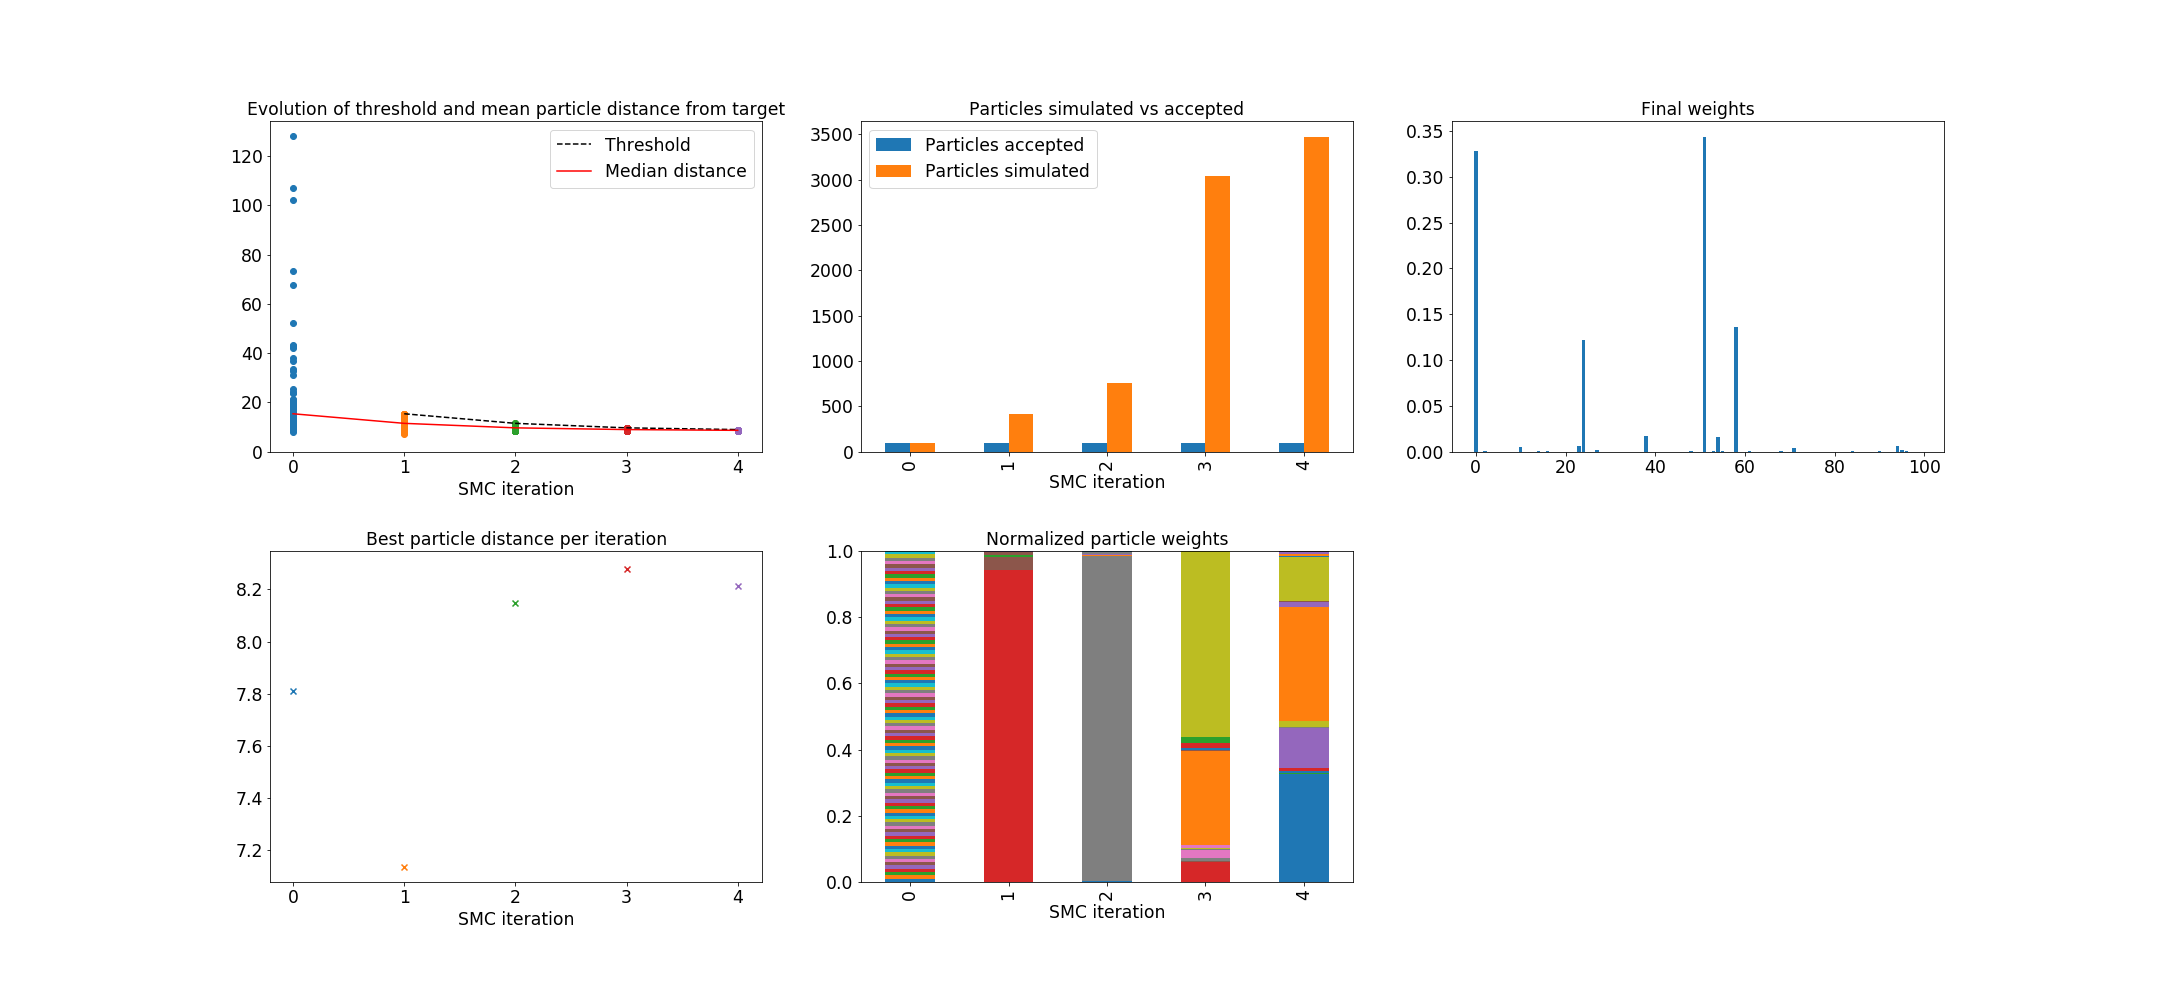
\includegraphics[width=\linewidth, scale=1]{images/abcsmc_statistics.jpg}
  \caption{ABC-SMC run statistics. We notice the distances of particles quickly decrease and converge to a value of approximately 6.6, which seems to be the minimum attainable using this model parametrization. We also notice an increasing number of particles simulated in order to fill the required population, but remains in the thousands. The total run-time is about 1h30 on a somewhat powerful personal computer.}
  \label{fig:abcsmc_statistics}
\end{figure}

\begin{figure}
  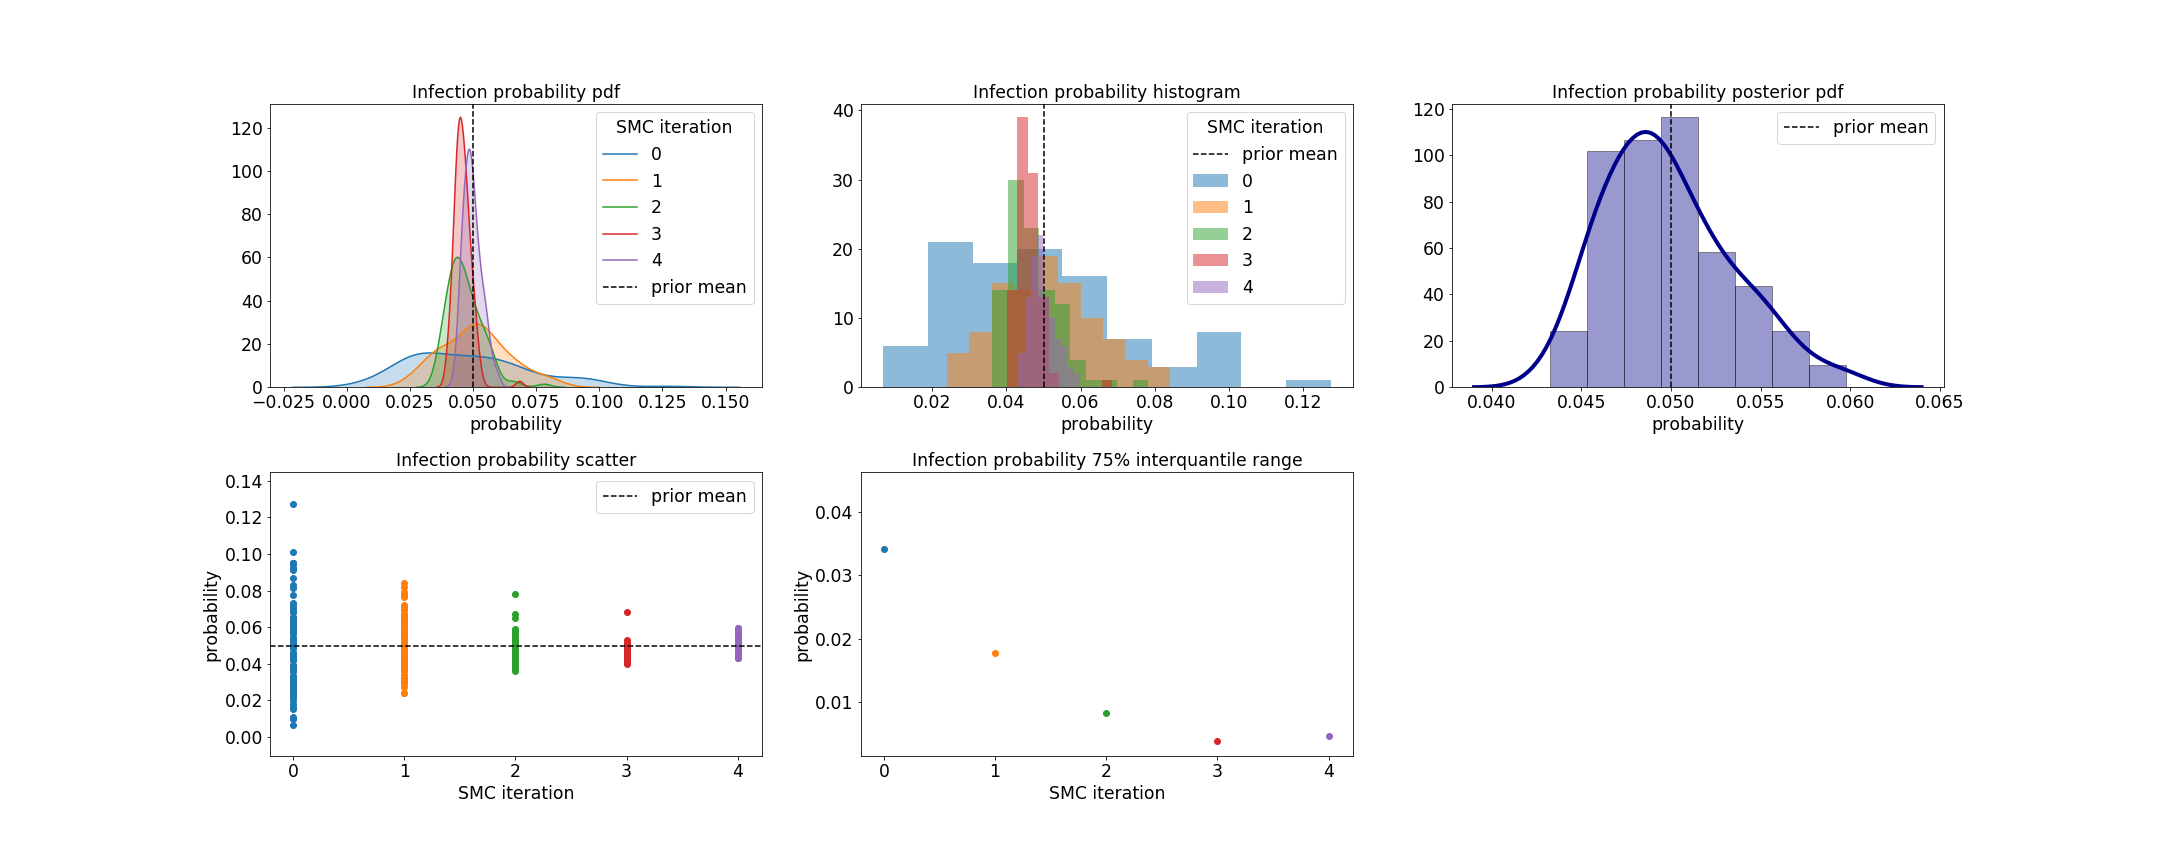
\includegraphics[width=\linewidth, scale=1]{images/inferred_infection_probability.jpg}
  \caption{Inferrence results for infection probability. We observe that each intermediate distribution becomes more and more peaked and concentrated around what seems to be the posterior value, as evidenced by a converging interquantile range. The resulting approximation of the posterior distribution is peaking at $5.3\%$, very close to our prior. We observe similarly good convergence for the other inferred parameters.}
  \label{fig:inferred_infection_probability}
\end{figure}

\begin{thebibliography}{9}
\bibitem{ABCSMC} 
Tina Toni, David Welch, Natalja Strelkowa, Andreas Ipsen and Michael P.H Stumpf, Approximate Bayesian computation scheme for parameter inference and model selection in dynamical systems, J. R. Soc. Interface.6187–202
\\\texttt{http://doi.org/10.1098/rsif.2008.0172}

\bibitem{ABC}
Mark A. Beaumont, Wenyang Zhang and David J. Balding, Approximate Bayesian Computation in Population Genetics, GENETICS December 1, 2002 vol. 162 no. 4 2025-2035 \\\texttt{https://www.genetics.org/content/162/4/2025}
\end{thebibliography}

\end{document}